\section{Hausdorff distance}
\label{hausdorff_distance_chapter}
\nblink{brats/15a\_hausdorff\_distance.ipynb}

In the previous section, we showed differences between the reference neural network output and the output of images where a part of them has been masked by a circle.
Showing this difference for all the applied masks is impractical, a single visualization which shows all the output segment changes would be helpful.
A first step is getting a single number for the difference of the two segments (unchanged reference segment, output segment from masked image).

A way to calculate the similarity (or difference) between two matrices (the output segments of the neural network are 2D matrices) is a distance function.

We choose the Hausdorff distance function because it has a specific property that is helpful for our requirements: A slightly moved object is still considered more similar to
an object with a completely different shape, even when the changed pixel count is exactly the same.

The formula for the Hausdorff distance is:
$ _{\mathrm {H} }(X,Y)=\max\{\,\sup _{x\in X}\inf _{y\in Y}d(x,y),\,\sup _{y\in Y}\inf _{x\in X}d(x,y)\} $

$X$ and $Y$ are the two sets/matrices which are compared. $d(x,y)$ is the distance between two points. $inf$ and $sup$ are the Infimum and supremum: When comparing two
ordered sets A and B, the infinum of A in comparision to B is the smallest TODO . A visualization

\begin{figure}[H]
\centering
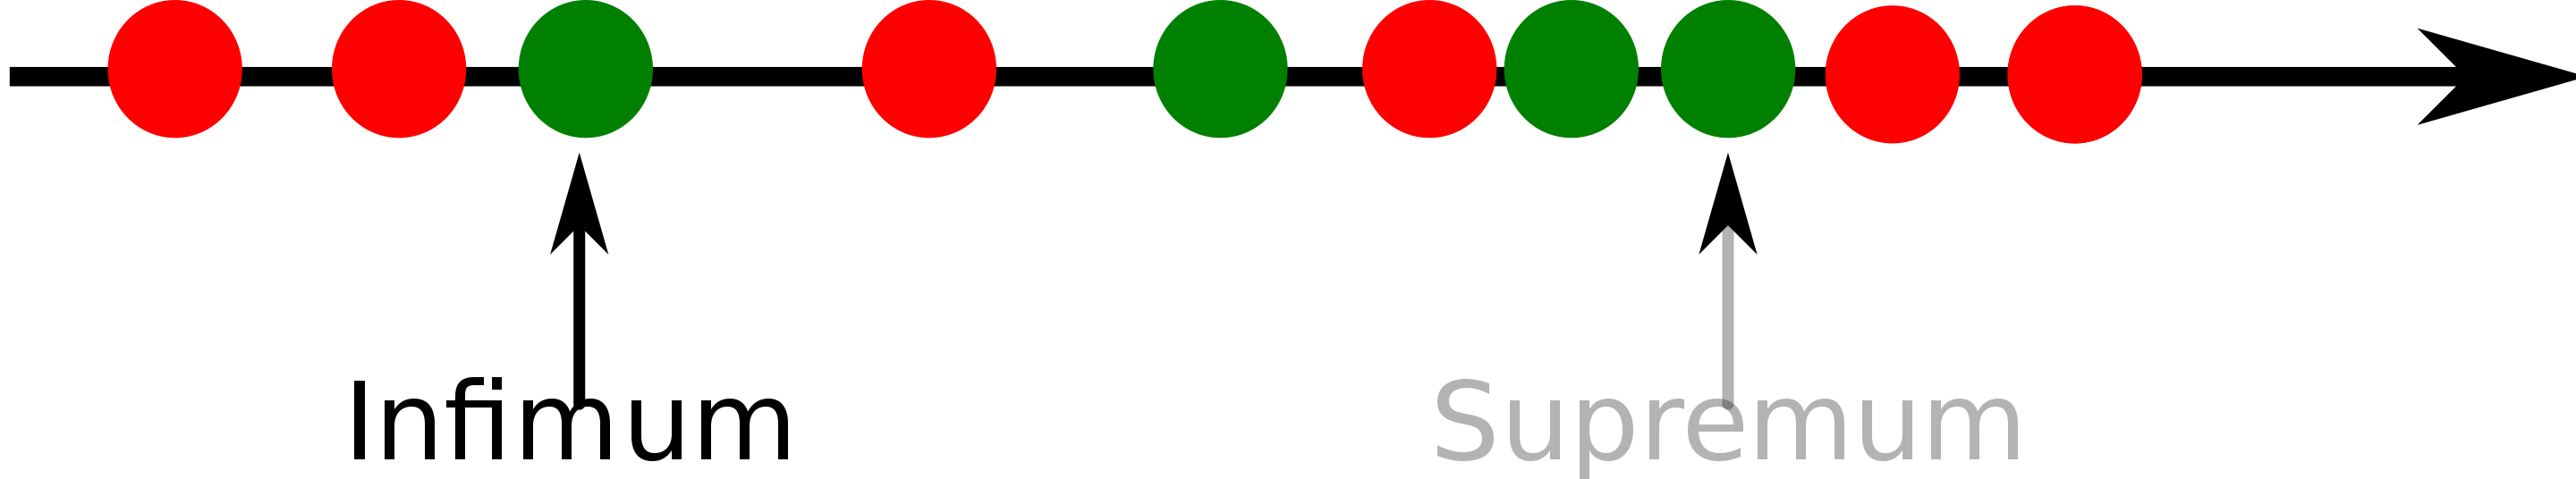
\includegraphics[width=8cm]{chapters/06_hdm/images/inf_sup.png}
\caption{Visualization of the Infimum and supremum \cite{hausdorffdistanceimage2}}
\label{inf_sup}
\end{figure}

Intuitively, the Hausdorff distance searches two different maximal distances between two sets and returns the higher one as the distance.
The maximal distance from set A to set B is the biggest distance between a pixel from set A to a pixel in set B, but the distance from the pixel from set A to the pixel B has to be the smallest distance from pixel A to any pixel on the set B.

A visual explanation of the Hausdorff distance is given in Figure \ref{hausdorff_distance}.

\begin{figure}[H]
\centering
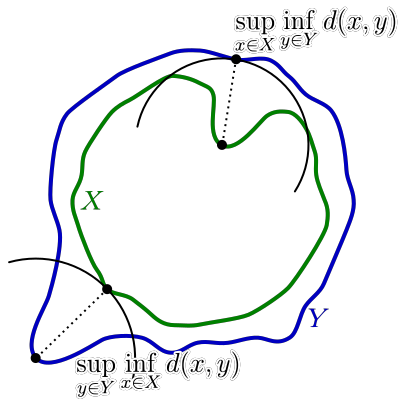
\includegraphics[width=8cm]{chapters/06_hdm/images/hausdorff_distance.png}
\caption{Visualization of the Hausdorff distance. The distance from set Y to set X is the maximal distance of a point on set Y to a point X \cite{hausdorffdistanceimage}}
\label{hausdorff_distance}
\end{figure}

\subsection{Examples}
\begin{figure}[H]
    \centering
    \begin{subfigure}{.5\textwidth}
        \centering
        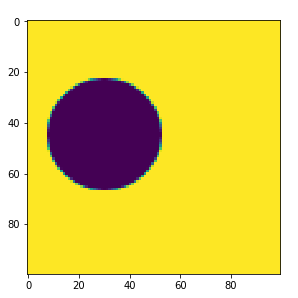
\includegraphics[width=.75\linewidth]{chapters/06_hdm/images/hdm_original.png}
        \caption{Original shape}
    \end{subfigure}%
    \begin{subfigure}{.5\textwidth}
        \centering
        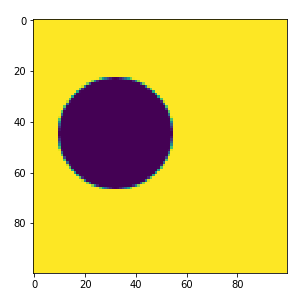
\includegraphics[width=.75\linewidth]{chapters/06_hdm/images/hdm_moved1.png}
        \caption{Shape moved slightly to the right}
    \end{subfigure}
    \caption{Hausdorff distance between the left and the right figure: 476. }
    \label{hdm_moved1}
\end{figure}


\begin{figure}[H]
    \centering
    \begin{subfigure}{.5\textwidth}
        \centering
        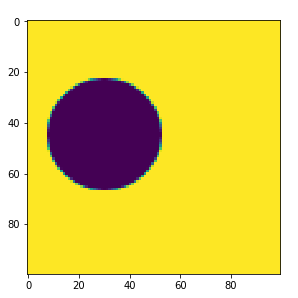
\includegraphics[width=.75\linewidth]{chapters/06_hdm/images/hdm_original.png}
        \caption{Original shape}
    \end{subfigure}%
    \begin{subfigure}{.5\textwidth}
        \centering
        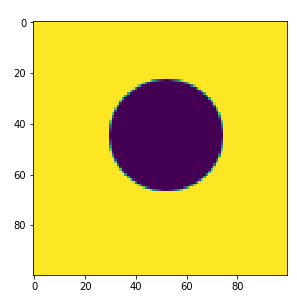
\includegraphics[width=.75\linewidth]{chapters/06_hdm/images/hdm_moved2.png}
        \caption{Shape moved to the right}
    \end{subfigure}
    \caption{Hausdorff distance between the left and the right figure: 1656. }
    \label{hdm_moved2}
\end{figure}

\begin{figure}[H]
    \centering
    \begin{subfigure}{.5\textwidth}
        \centering
        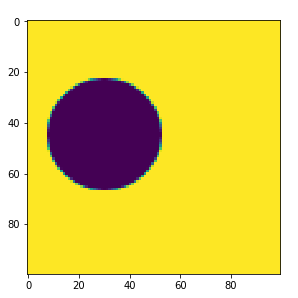
\includegraphics[width=.75\linewidth]{chapters/06_hdm/images/hdm_original.png}
        \caption{Original shape}
    \end{subfigure}%
    \begin{subfigure}{.5\textwidth}
        \centering
        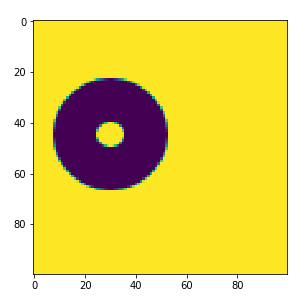
\includegraphics[width=.75\linewidth]{chapters/06_hdm/images/hdm_hole.png}
        \caption{Shape moved to the right}
    \end{subfigure}
    \caption{Hausdorff distance between the left and the right figure: 840. }
    \label{hdm_hole}
\end{figure}

\begin{figure}[H]
    \centering
    \begin{subfigure}{.5\textwidth}
        \centering
        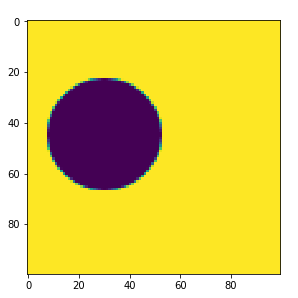
\includegraphics[width=.75\linewidth]{chapters/06_hdm/images/hdm_original.png}
        \caption{Original shape}
    \end{subfigure}%
    \begin{subfigure}{.5\textwidth}
        \centering
        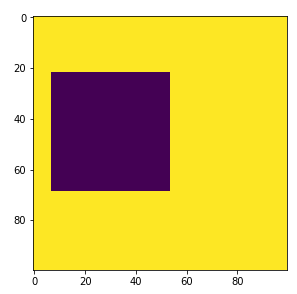
\includegraphics[width=.75\linewidth]{chapters/06_hdm/images/hdm_square.png}
        \caption{Shape moved to the right}
    \end{subfigure}
    \caption{Hausdorff distance between the left and the right figure: 1197. }
    \label{hdm_square}
\end{figure}


\begin{figure}[H]
    \centering
    \begin{subfigure}{.5\textwidth}
        \centering
        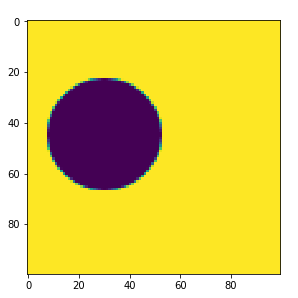
\includegraphics[width=.75\linewidth]{chapters/06_hdm/images/hdm_original.png}
        \caption{Original shape}
    \end{subfigure}%
    \begin{subfigure}{.5\textwidth}
        \centering
        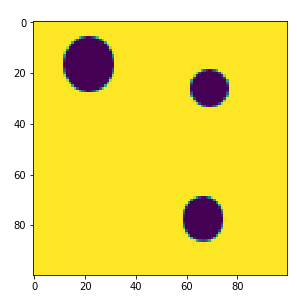
\includegraphics[width=.75\linewidth]{chapters/06_hdm/images/hdm_smaller_circles.png}
        \caption{Shape moved to the right}
    \end{subfigure}
    \caption{Hausdorff distance between the left and the right figure: 1353. }
    \label{hdm_smaller_circles}
\end{figure}
